\chapter{Data acquisition for CHIPS} %%%%%%%%%%%%%%%%%%%%%%%%%%%%%%%%%%%%%%%%%%%%%%%%%%%%%%%%%%%%%
\label{chap:daq} %%%%%%%%%%%%%%%%%%%%%%%%%%%%%%%%%%%%%%%%%%%%%%%%%%%%%%%%%%%%%%%%%%%%%%%%%%%%%%%%%

The primary task of any Data Acquisition (DAQ) system is the processing of low-level signals
measuring real-world physics and their transfer to permanent storage for further analysis.
Commonly, this procedure also includes decision making as to whether the signal is deemed
interesting enough to record, known as a \emph{trigger}. Both these tasks can make DAQ systems
incredibly complex, especially when they must operate in an efficient and resilient manner for
vast amounts of data in real-time, while also providing detector control and monitoring.

In the context of the \chips project, the DAQ system records all PMT hits, timestamps them using a
common clock, and transfers them out of the detector to a central processing node. This node then
applies a trigger to select hits that fall within the interesting \numi beam spill time window.
All selected hits are then sliced into events and moved to permanent storage for further analysis.
Alongside these processes, the DAQ also configures the detector and provides data quality and
detector component monitoring.

Although relatively simple when compared to the incredibly complex and time-pressured DAQ systems
of the LHC experiments, the DAQ system developed for the \chips project introduces some novel
approaches to solve the unique constraints of the \chips concept. Namely, deployment within a body
of water and a limited resource budget. In this chapter, the DAQ system for \chips as applied to
the \chipsfive prototype detector module is described alongside highlighting any novel approaches.
The description is presented in two broad categories, hardware and software, with a short
description of the timing system beforehand.

\section{White Rabbit timing} %%%%%%%%%%%%%%%%%%%%%%%%%%%%%%%%%%%%%%%%%%%%%%%%%%%%%%%%%%%%%%%%%%%%
\label{sec:daq_timing} %%%%%%%%%%%%%%%%%%%%%%%%%%%%%%%%%%%%%%%%%%%%%%%%%%%%%%%%%%%%%%%%%%%%%%%%%%%

To ensure PMT hit times are synchronised throughout \chips detectors, a common clock must be
shared across all timestamping electronics. For this purpose, \chips employs a \emph{White Rabbit}
(WR) network~\cite{lipinski2011}. Initially developed at CERN, the open-source WR project provides
an ethernet-based time distribution network with sub-nanosecond synchronisation accuracy between
nodes. By using two-way exchanges of WR messages, precise adjustment of individual node clock
phases and offsets is possible across thousands of devices, separated by tens of kilometres. All
of this is achieved in parallel with a standard data transfer network capable of
\unit{1}{\text{Gb}} speeds.

All nodes are synchronised to the clock of a \emph{GrandMaster} node which is typically a WR
\emph{switch}, the most common WR hardware component. As input, the switch receives an IRIG-B
(Inter-Range Instrumentation Group timecode B) and a \unit{10}{\text{MHz}} signal from a GPS
disciplined oscillator. These inputs allow for the WR network clock to be synchronised to
International Atomic Time (TAI). As \chips detector modules require synchronisation to accelerator
clocks many hundreds of kilometres in order to determine the arrival time of beam spills
accurately, this timing is particularly important.

WR hardware is commercially available from many vendors. Within \chipsfive, two WR devices are
used for time synchronisation and data transfer, both shown in Fig.~\ref{fig:wr_electronics}.
Firstly, a compact version of the standard WR switch~\cite{wrswitch2020}, specially developed for
the \chips project at Nikhef~\cite{wrchromium2020}. Secondly, a WR-LEN (Lite Embedded Node) from
Seven Solutions~\cite{wrlen2020}. All WR components are connected using \unit{1}{\text{Gb}}
bi-directional optical fibre connections using the \unit{1310}{\text{nm}} and
\unit{1550}{\text{nm}} wavelengths via Small Form-Factor Pluggable Transceivers (SFPs).

\begin{figure} % WHITE-RABBIT COMPONENTS DIAGRAM %
    \centering
    \subcaptionbox{White Rabbit switch}{%
        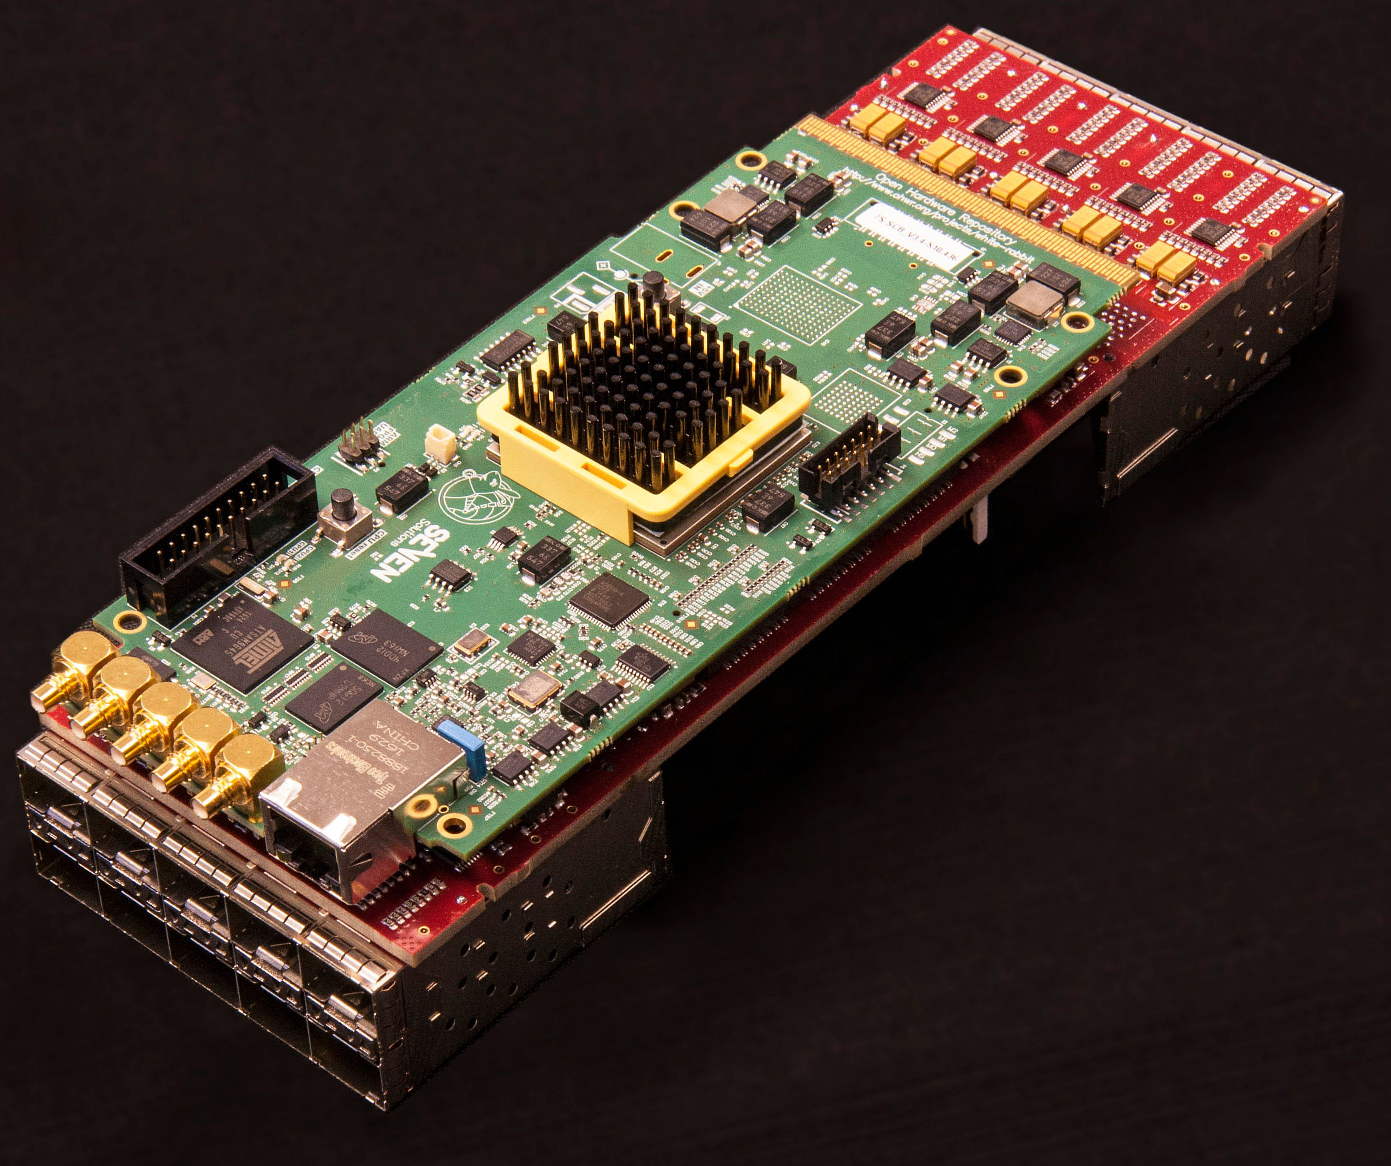
\includegraphics[height=6cm]{diagrams/5-daq/wr_switch.pdf}%
    }
    \quad
    \subcaptionbox{White Rabbit LEN}{%
        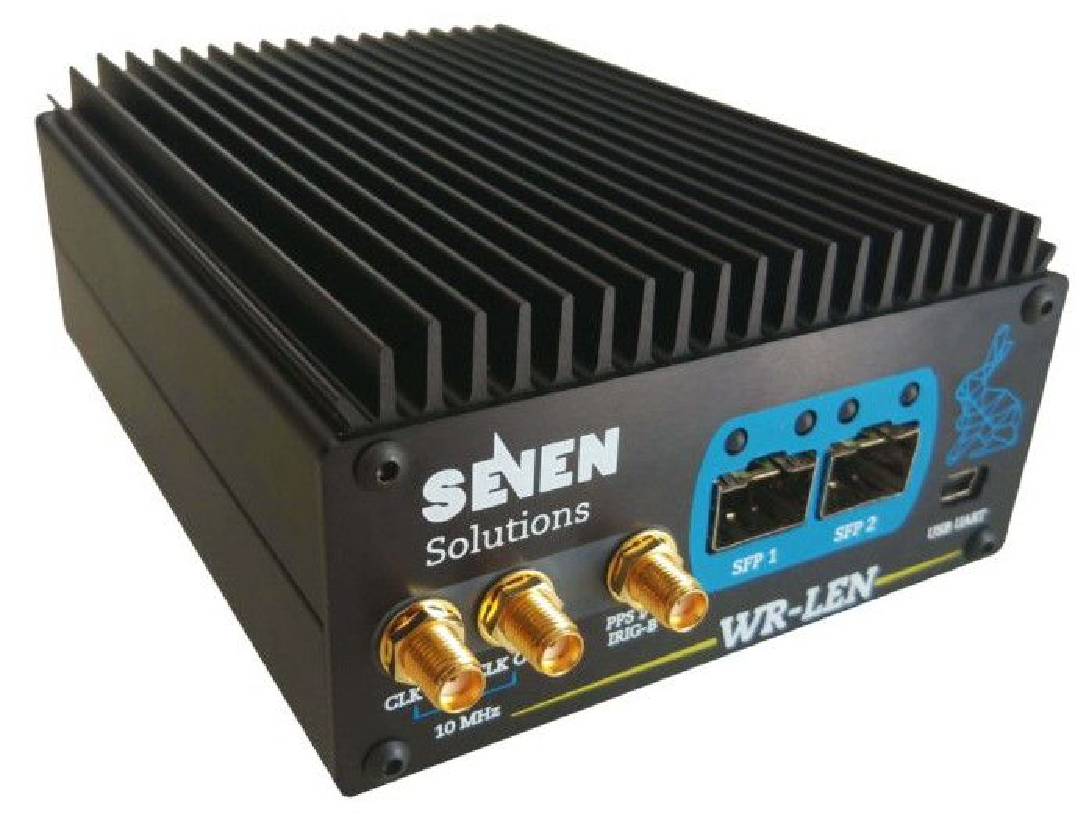
\includegraphics[height=6cm]{diagrams/5-daq/wr_len.pdf}%
    }
    \caption[Pictures of the White Rabbit timing hardware used within \chipsfive.]
    {Pictures of the White Rabbit timing hardware used within \chipsfive. The compact White rabbit
        switch  specially designed for \chips is shown in (a), while the White Rabbit Lite
        Embedded Node (WR-LEN) from Seven Solutions is shown in (b).}
    \label{fig:wr_electronics}
\end{figure}

Fig.~\ref{fig:sync} shows the WR synchronised Pulse Per Second (PPS) clock rising edges for two
\chipsfive WR switches separated by \unit{500}{\text{m}} of fibre. With the vertical ticks
representing single nanoseconds, sub-nanosecond time synchronisation accuracy between the switches
is achieved.

\begin{figure} % WHITE-RABBIT SYNC DIAGRAM %
    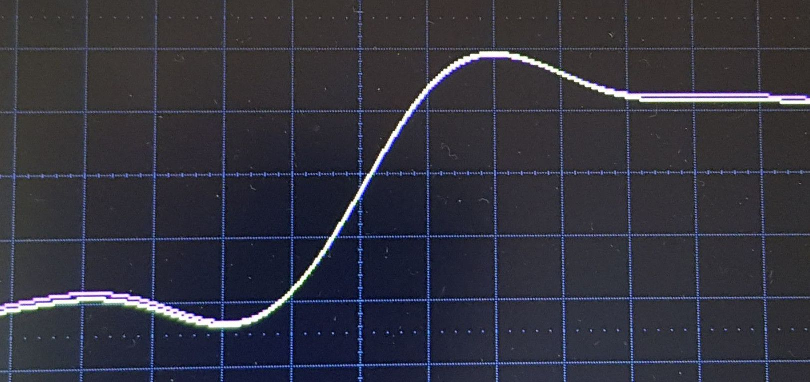
\includegraphics[width=0.7\textwidth]{diagrams/5-daq/sync.pdf}
    \caption[Picture of White Rabbit timing synchronisation seen in \chips.]
    {Picture of an oscilloscope measuring the PPS output signal from two WR switches shown in pink
        and yellow at either end of a \unit{500}{\text{m}} long optical fibre. The vertical
        ticks are in nanoseconds showing the sub-nanosecond synchronisation possible with the WR
        timing network.}
    \label{fig:sync}
\end{figure}

\section{Hardware} %%%%%%%%%%%%%%%%%%%%%%%%%%%%%%%%%%%%%%%%%%%%%%%%%%%%%%%%%%%%%%%%%%%%%%%%%%%%%%%
\label{sec:daq_hard} %%%%%%%%%%%%%%%%%%%%%%%%%%%%%%%%%%%%%%%%%%%%%%%%%%%%%%%%%%%%%%%%%%%%%%%%%%%%%

The hardware of the \chipsfive DAQ system is split into two distinct implementations at its lower
levels (closest to the PMTs), corresponding to the Nikhef and Madison \textsc{Pom} types. \chips R\&D
efforts have developed the novel Madison implementation with the view to use this hardware within
detector modules exclusively. However, as a safe stepping stone, while development and testing are
still ongoing, \chipsfive mainly contains proven Nikhef hardware developed initially for the
KM3NeT experiment~\cite{adrian2016}.

The complete DAQ and power distribution system for \chipsfive is diagrammatically shown in
Fig.~\ref{fig:daq}. The following subsections describe each component, starting from the lowest
level and working upwards. The Nikhef and Madison descriptions are separated for clarity as well
as the high-level combined hardware systems, part of which is not physically located within the
detector but onshore in an electronics hut (different from the water filtration hut).

\begin{figure} % DAQ DIAGRAM %
    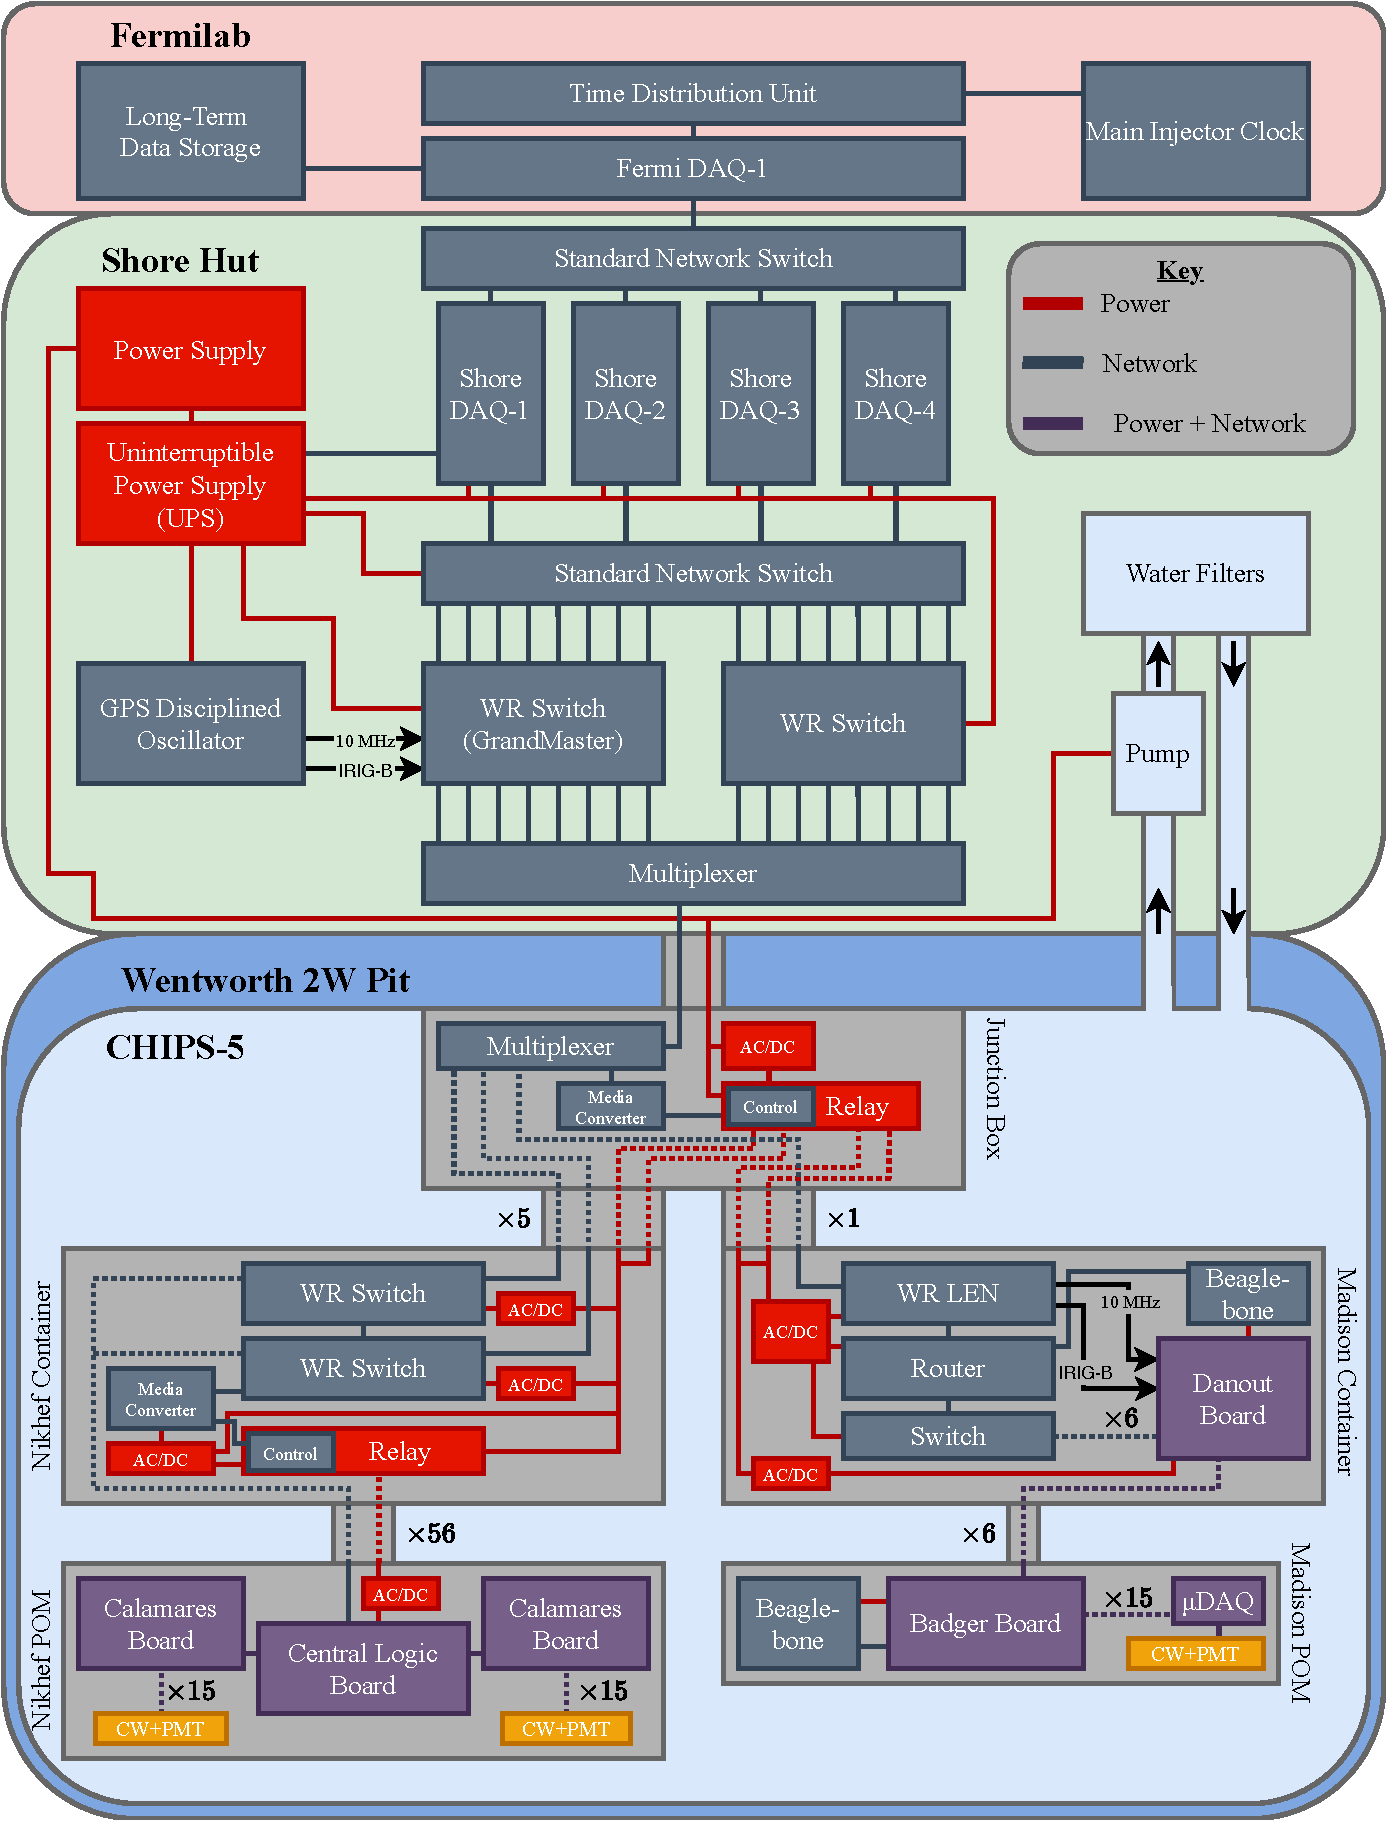
\includegraphics[width=\textwidth]{diagrams/5-daq/daq.pdf}
    \caption[Diagram of the complete \chipsfive data acquisition and power distribution system.]
    {Diagram of the complete \chipsfive DAQ and power distribution system.}
    \label{fig:daq}
\end{figure}

Common to both low-level hardware implementations is the use of the Time over Threshold (ToT)
method for PMT signal digitisation. Each analogue PMT pulse is fed to a ToT discriminator coupled
with a Time to Digital Converter (TDC) in order to generate a digitised recorded hit, as
illustratively shown in Fig.~\ref{fig:tot}. Even though ToT values are less accurate and do not
scale linearly with deposited charge, they are used instead of the more common Analogue to Digital
Converter (ADC) readout as the electronics are simpler and notably cheaper.

\begin{figure} % TOT DIAGRAM DIAGRAM %
    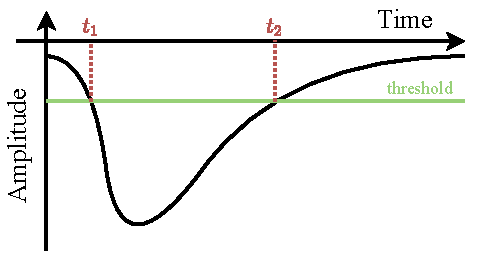
\includegraphics[width=0.6\textwidth]{diagrams/5-daq/tot.pdf}
    \caption[Illustrative diagram showing how Time over Threshold is measured.]
    {Illustrative diagram showing how a ToT value is measured. As soon as the rising edge of a PMT
        charge pulse rises above a given threshold (goes below in the negative charge case) a time
        is recorded $t_{1}$, when the falling edge later falls below the threshold a second time
        $t_{2}$ is recorded. The difference in time between $t_{1}$ and $t_{2}$ is output by the
        electronics as a digitised ToT value.}
    \label{fig:tot}
\end{figure}

\subsection{Nikhef hardware} %%%%%%%%%%%%%%%%%%%%%%%%%%%%%%%%%%%%%%%%%%%%%%%%%%%%%%%%%%%%%%%%%%%%%
\label{sec:daq_hard_Nikhed} %%%%%%%%%%%%%%%%%%%%%%%%%%%%%%%%%%%%%%%%%%%%%%%%%%%%%%%%%%%%%%%%%%%%%%

All Nikhef HZC PMTs are attached directly to a simple readout board containing a high-voltage
generating Cockcroft-Walton circuit. Up to 30 such PMTs are connected to two \emph{Calamares}
boards within the electronics box of each Nikhef \textsc{Pom} via standard category 5 cables with
RJ45 connectors, as shown in Fig.~\ref{fig:nikhef_plane}. Both Calamares boards are directly
attached to a Central Logic Board (CLB)~\cite{biagi2015, eijk2015}. The CLB contains ToT
discriminators and TDCs to digitise the recorded PMT signals as well as electronics to synchronise
to the WR network clock for timestamping. Each Nikhef \textsc{Pom} electronics box also contains
an AC to DC power converter (AC/DC) whose output is fed into the CLB for distribution.

\begin{figure} % NIKHEF PLANE DIAGRAM %
    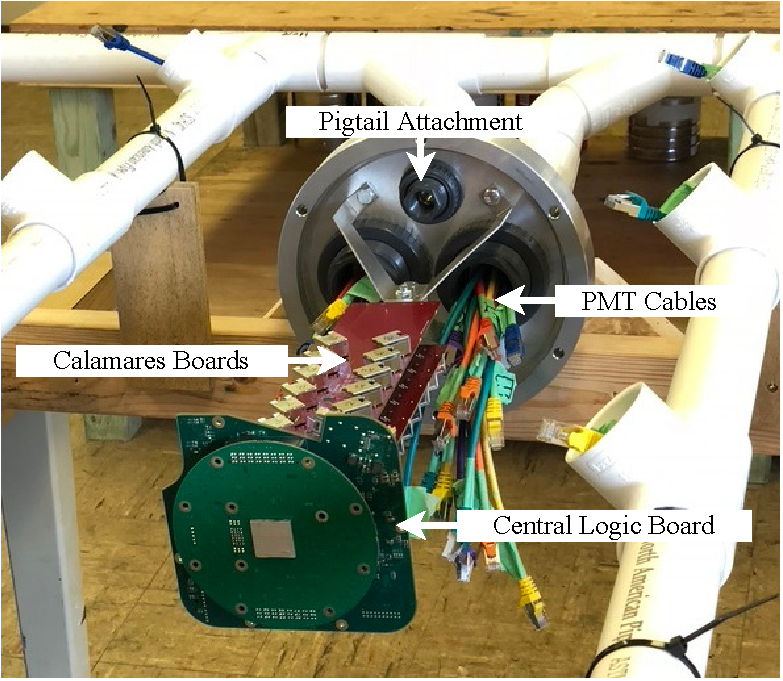
\includegraphics[width=0.8\textwidth]{diagrams/5-daq/nikhef_plane.pdf}
    \caption[Labelled picture of the Nikhef \textsc{Pom} electronics box.]
    {Labelled picture of the Nikhef \textsc{Pom} electronics box. Both ends of the category 5 PMT cables
        can be seen, either at the PMT mounting points or entering the electronics box and not yet
        plugged into Calamares boards.}
    \label{fig:nikhef_plane}
\end{figure}

Every Nikhef \textsc{Pom} is connected via a single optical fibre and a single power connection to a
\emph{Nikhef-container}, the contents of which are labelled in the bottom half of
Fig.~\ref{fig:full_setup}. Two WR switches are used within each container to provide sufficient
\textsc{Pom} networking ports. Both are powered by independent AC to DC converters and connected via a
single optical fibre each to the higher level DAQ systems. An additional connection between each
switch ensures that if one higher-level connection fails the other can still be used.

Each Nikhef-container also contains a relay board to control the power supply to individual \textsc{Pom}s.
The relay board control electronics are powered via an AC to DC converter and connected to one of
the switches via a media converter for networking. The media converter is required to convert the
optical fibre (1000BASE ethernet) WR switch connection to a standard RJ45 copper cable (100BASE
ethernet). A total of five Nikhef-containers are present within \chipsfive.

\begin{figure} % FULL SETUP DIAGRAM %
    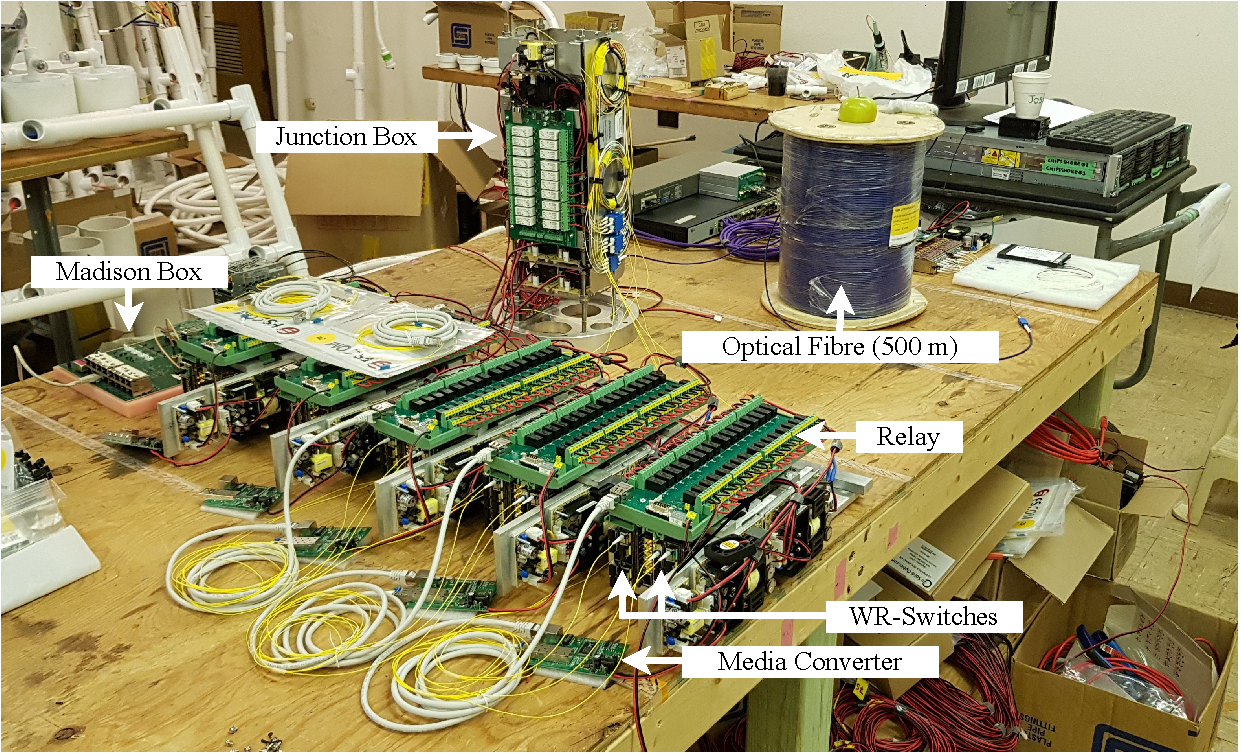
\includegraphics[width=\textwidth]{diagrams/5-daq/full_setup.pdf}
    \caption[Picture of the non \textsc{Pom} components of the \chipsfive DAQ system]
    {Picture of the non \textsc{Pom} components of the \chipsfive DAQ system arranged on a table at the
        PolyMet mining administration building.}
    \label{fig:full_setup}
\end{figure}
\subsection{Madison hardware} %%%%%%%%%%%%%%%%%%%%%%%%%%%%%%%%%%%%%%%%%%%%%%%%%%%%%%%%%%%%%%%%%%%%
\label{sec:daq_hard_madison} %%%%%%%%%%%%%%%%%%%%%%%%%%%%%%%%%%%%%%%%%%%%%%%%%%%%%%%%%%%%%%%%%%%%%

Every Madison Hamamatsu PMT is directly attached to a high-voltage generating Cockcroft-Walton
board followed by a signal processing \emph{$\mu$DAQ}, as shown in
Fig.~\ref{fig:madison_pmt_assembly}. The $\mu$DAQ is a small microcontroller developed for both
IceCube and \chips at WIPAC in Madison. Capable of timestamping and digitising signals directly at
the PMT level, the $\mu$DAQ also sets the PMT operating voltage by controlling the
Cockcroft-Walton board~\cite{eijk2018}.

Up to 16 $\mu$DAQs receive power, networking, and IRIG-B and \unit{10}{\text{MHz}} timing
signals from a \emph{badger-board}, as shown in Fig.~\ref{fig:madison_plane}. Standard category 5
cables with RJ45 connectors are used. The badger-board is located within the electronics box of
each Madison \textsc{Pom} and acts as a simple fanout and power control board. For logic, each badger-board
has an attached mezzanine Beaglebone~\cite{beagle2020}. This single-board Linux machine (very
similar to a Raspberry Pi) controls the power supply to and receives hits from the attached
$\mu$DAQs.

\begin{figure} % MADISON PLANE DIAGRAM %
    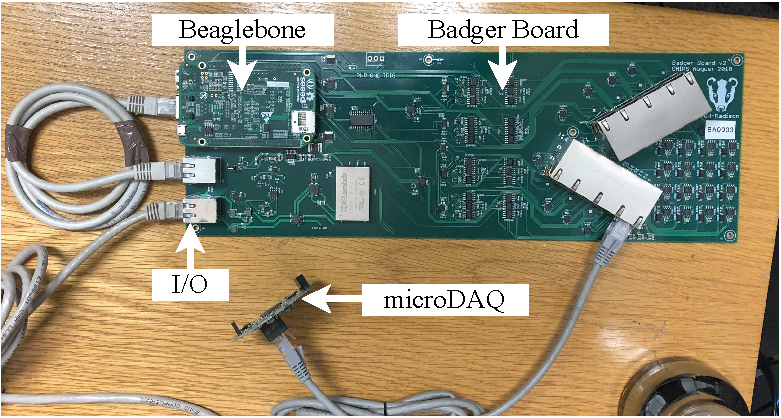
\includegraphics[width=0.8\textwidth]{diagrams/5-daq/madison_plane.pdf}
    \caption[Labelled picture of the components of the Madison \textsc{Pom} electronics box.]
    {Labelled picture of the components of the Madison \textsc{Pom} electronics box.}
    \label{fig:madison_plane}
\end{figure}

Similarly, up to 16 Madison \textsc{Pom} badger-boards receive power, networking and IRIG-B and
\unit{10}{\text{MHz}} timing signals from a \emph{danout-board} located within a single
\emph{Madison-container}. Again, standard category 5 cables with RJ45 connectors are used. The
full contents of the Madison-container are shown in Fig.~\ref{fig:madison_box}. Similar to the
badger-board, the danout-board acts as a simple fanout and power control board with an attached
mezzanine Beaglebone. However, in this case, the attached Beaglebone acts only to control the
power provided by the danout-board.

PMT hits and other packets are instead routed through the danout-board into a networking stack.
Consisting of a WR-LEN, a router (required due to the limited WR-LEN routing table size), and a
switch, the stack provides networking to the higher-level DAQ via a single optical fibre. The WR
clock synchronised IRIG-B and \unit{10}{\text{MHz}} timing signals are output by the WR-LEN to
the danout-board for forwarding to the lower-level components. Additionally, two AC to DC
converters provide power for both the devices within the container and all lower-level components
via the danout-board.

\begin{figure} % MADISON BOX DIAGRAM %
    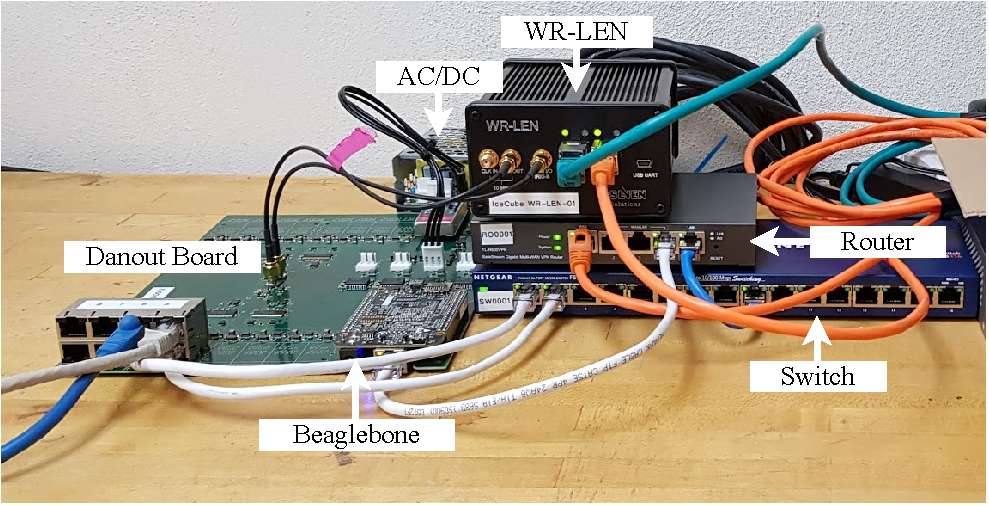
\includegraphics[width=\textwidth]{diagrams/5-daq/madison_box.pdf}
    \caption[Labelled picture of the Madison-container components.]
    {Labelled picture of the Madison-container components. The blue and grey cables exiting the
        left hand side of the image go to individual Madison \textsc{Pom}s connecting to the I/O port shown
        in fig.~\ref{fig:madison_plane}. An optical fibre connection into the left SFP port of the
        WR-LEN is used in reality rather than the copper connection shown here.}
    \label{fig:madison_box}
\end{figure}

- Can reference the Nikhef stuff that I have already described - THIS IS WHAT ALL FUTURE CHIPS
DETECTOR SHOULD USE FULLY!!! - This is the novel stuff that is much cheaper! NOVEL NOVEL NOVEL
CHEAP CHEAP CHEAP SIMPLE SIMPLE SIMPLE COMMERCIAL COMMERCIAL COMMERCIAL CAPABLE CAPABLE CAPABLE
LINUX LINUX LINUX Can configure at a later data as we have a full linux machine at a very low
level of the DAQ system. Can do lots of processing close to where the DAQ inputs are created.
unlike in the Nikhef case where it is done on the CLB. As the beaglebone is a full linux machine
at a low level lots of processing can occur close to the PMTs. It controls the power and
networking on the $\mu$DAQ, receives their hits before forwarding further up the chain. The
$\mu$DAQ and beaglebone are novel approaches, CHEAP, more processing close to PMTs!!! commercially
available!! - Can introduce additional logic once deployed via simple software updates to the
beaglebone.

\subsection{Combined systems} %%%%%%%%%%%%%%%%%%%%%%%%%%%%%%%%%%%%%%%%%%%%%%%%%%%%%%%%%%%%%%%%%%%%
\label{sec:daq_hard_combined} %%%%%%%%%%%%%%%%%%%%%%%%%%%%%%%%%%%%%%%%%%%%%%%%%%%%%%%%%%%%%%%%%%%%

Each Nikhef-container and Madison-container is connected to the \chipsfive \emph{junction-box},
labelled in Fig.~\ref{fig:full_setup}. This central container acts as the interface between the
detector electronics and the umbilical carrying data and power between the shore and the detector.
All connections to the junction-box (as well as those between \textsc{Pom}s and Nikhef and Madison
containers) are made within watertight, flexible PVC tubing called \emph{manifolds}. These tubes
span all corners of the \chipsfive detector, as shown in Fig.~\ref{fig:manifold}.

\begin{figure} % MANIFOLD DIAGRAM %
    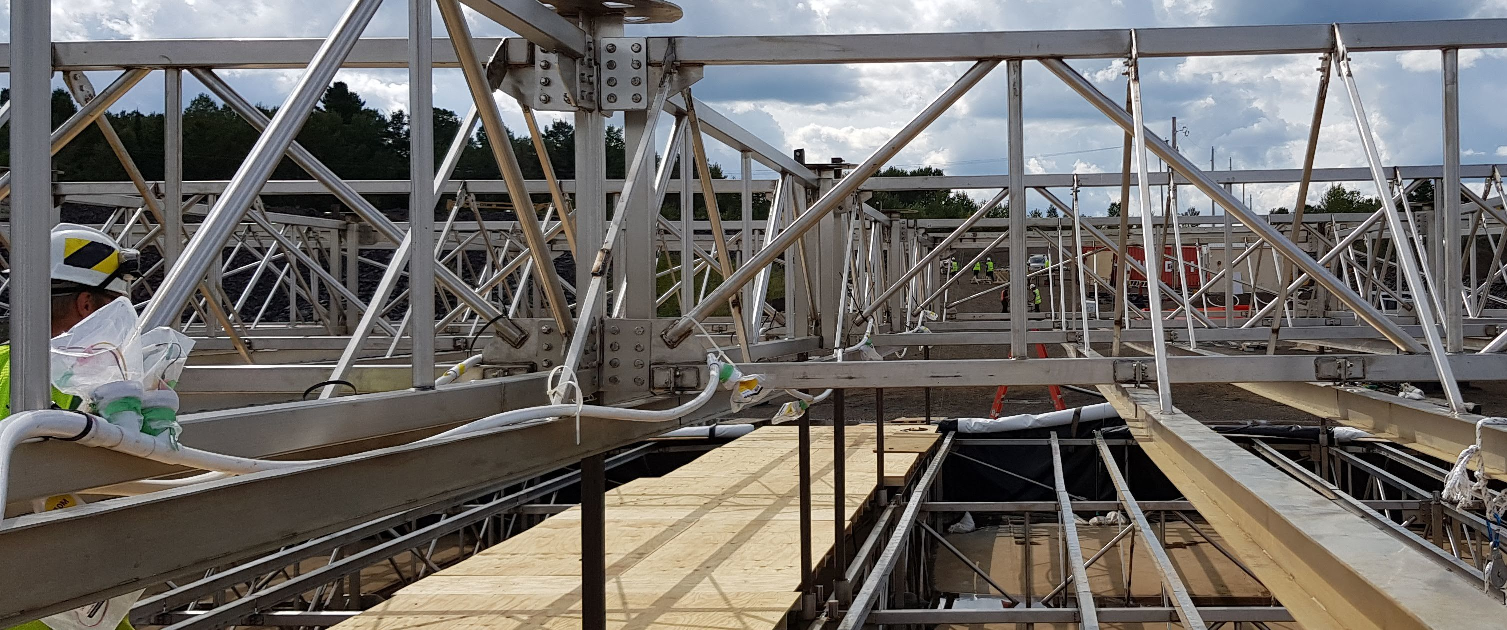
\includegraphics[width=\textwidth]{diagrams/5-daq/manifold.pdf}
    \caption[manifold short]
    {Picture of a Nikhef \textsc{Pom} to Nikhef-container manifold (in white) attached to the top-cap of
        the \chipsfive detector. In the left of the image, two unattached Nikhef \textsc{Pom} pigtail
        connections are seen, both covered in green tape and a plastic bag.}
    \label{fig:manifold}
\end{figure}

For networking the junction-box contains a Coarse Wavelength Division Multiplexing (CWDM)
multiplexer/demultiplexer (MUX/DEMUX). This device supports 32 wavelengths for a total of 16
bi-directional \unit{1}{\text{Gb}} connections over the single \unit{500}{\text{m}} long
umbilical optical fibre. Each WR-LEN or WR switch within the detector uses one of these channels
exclusively with the corresponding wavelength SFP.

The umbilical power connections are distributed via two thick copper plates to all the relay
channels within the junction-box. Two relay boards are used to provide a sufficient number of
output channels, with their control electronics powered by separate AC to DC converters and each
connected to one of the multiplexer/demultiplexer networking channels via a media converter. Each
relay channel also has a built-in \emph{trip gate} to immediately power-off the channel if a
current surge is detected. This protection is particularly important for \chips as water leaks are
possible.

The contents of the DAQ \emph{Shore Hut} next to the water filtration hut onshore are shown in
Fig.~\ref{fig:hut_daq}. The single umbilical optical fibre passes through a
multiplexer/demultiplexer before each of the wavelength-specific channels are passed into one of
two WR switches to provide sufficient bandwidth. Multiple Virtual Local Area Networks (VLANs) are
configured on each switch such that for each wavelength channel only a single corresponding port
on the other side of the switch carries data to a standard networking switch. Of the two WR
switches, one is configured to be the WR network GrandMaster with connections to a GPS disciplined
oscillator. A single connection is also made between the WR switches for synchronisation.

\begin{figure} % WHITE-RABBIT GM SETUP DIAGRAM %
    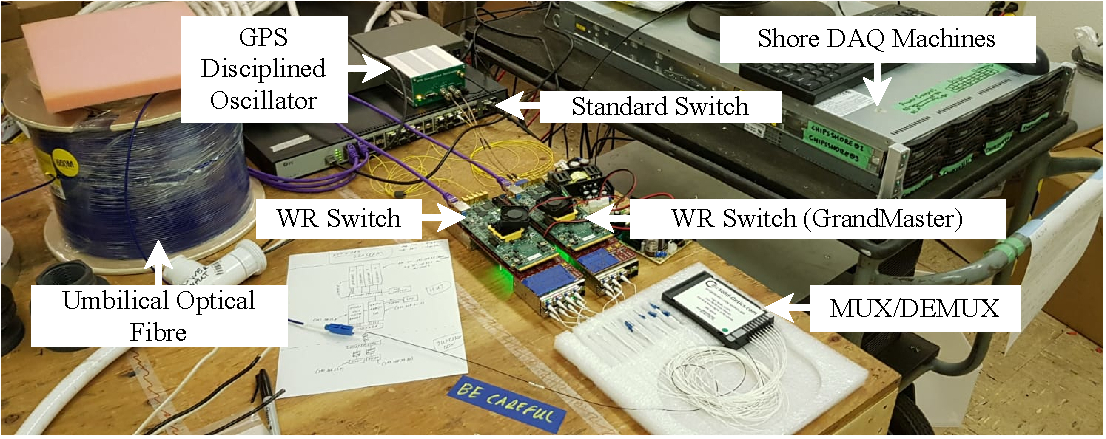
\includegraphics[width=\textwidth]{diagrams/5-daq/hut_daq.pdf}
    \caption[Picture of the onshore components of the \chipsfive DAQ system]
    {Picture of the onshore components of the \chipsfive DAQ system arranged on a table at the
        PolyMet mining administration building.}
    \label{fig:hut_daq}
\end{figure}

The standard network switch provides \unit{10}{\text{Gb}} connections to each of the Shore DAQ
computing machines whose specific roles are detailed in Section.~\ref{sec:daq_soft}. Each machine
is also connected to a second standard network router which provides a higher level \chips network
for non-DAQ related work, also provides connections to the broader internet for communication with
Fermilab.

An uninterruptible power supply provides power to all electronics within the Shore Hut, providing
power for up to \unit{15}{\text{minutes}} after a power cut (surprisingly quite common).

\section{Data flow and software} %%%%%%%%%%%%%%%%%%%%%%%%%%%%%%%%%%%%%%%%%%%%%%%%%%%%%%%%%%%%%%%%%
\label{sec:daq_soft} %%%%%%%%%%%%%%%%%%%%%%%%%%%%%%%%%%%%%%%%%%%%%%%%%%%%%%%%%%%%%%%%%%%%%%%%%%%%%

TODO: Write the software section of the DAQ chapter

~\cite{chipsdaq2020}

- What makes this implementation special
- Limited resource, but brilliant capabilities
- Use existing software when possible

- Need to talk about what is novel, new and exciting!
- Not so much about the hardcore electronics details, more high level
- FINITE STATE MACHINE!!!

SOFTWARE
- The beam spill
- Hit acquisition and handling
- Detector and data quality monitoring

\begin{figure} % SOFTWARE DIAGRAM %
    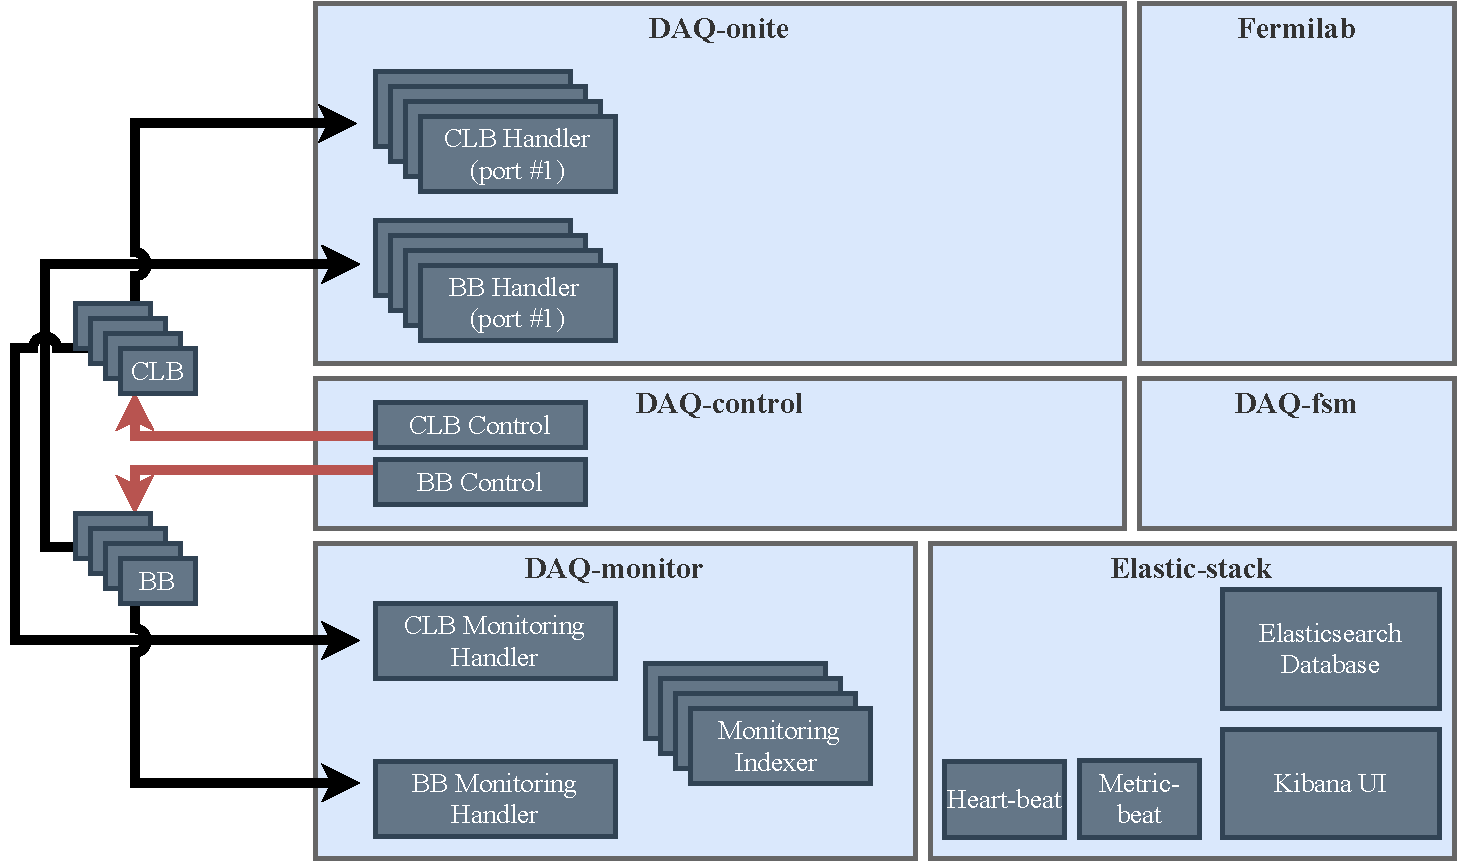
\includegraphics[width=\textwidth]{diagrams/5-daq/daq_software.pdf}
    \caption[daq software short]
    {daq software long}
    \label{fig:daq_software}
\end{figure}

- INCLUDE DATA RATES IN SOFTWARE DIAGRAM
- INCLUDE WHICH MACHINES THINGS RUN ON IN SOFTWARE DIAGRAM

- Where the DHCP server is
- Separated into slow-control, data collection, and

- Need to get across what makes this DAQ implementation special and novel, what are the
interesting unique bits of it? Limited resources but great performance! Use of existing hardware
and software! Modern approaches to doing things, good part of small collaboration!
- Needs to able to cope with 4 degrees at bottom!
- Talk about expected data through put, what we can cope with
- Jumbo frames etc

- An `all-data-to-shore' approach as done in KM3NeT
- Data is sent in UDP packets (not TCP so some will go missing)
- $\mu$DAQ software repository with fh-library (field-hub) novel communication library
in~\cite{microdaq2020}. Most of Madison code is written in c!
- Mainly written in C++, full asynchronous using the BOOST Asio library in~\cite{boost2020} which
is a library for network and low-level I/O programming using an asynchronous model.
- Taking inspiration from the KM3NeT DAQ Java software
- The detector is configured using a single human readable configuration file that defines all the
\textsc{Pom} types, MAC addresses, IP addresses, types, relay channels, which channels should be active and
their associate high voltage setting, threshold and electronic ID.
- Typical ethernet frame has a maximum transmission unit (MTU) size of 1500 bytes, we use Jumbo
frames that allow for an MTU of 9000 bytes, this means we have a lot less small frames with only a
limited number of recorded hits, which proved to be taxing to the switches and lead to an increase
in the number of dropped frames.
- 1Gb links between WR switches, 10Gb link between FS switch and main DAQ machine. Provides
sufficient bandwidth, DO A SMALL CALCULATION!

\subsection{Detector control} %%%%%%%%%%%%%%%%%%%%%%%%%%%%%%%%%%%%%%%%%%%%%%%%%%%%%%%%%%%%%%%%%%%%
\label{sec:daq_soft_control} %%%%%%%%%%%%%%%%%%%%%%%%%%%%%%%%%%%%%%%%%%%%%%%%%%%%%%%%%%%%%%%%%%%%%

\subsection{Hit acquisition} %%%%%%%%%%%%%%%%%%%%%%%%%%%%%%%%%%%%%%%%%%%%%%%%%%%%%%%%%%%%%%%%%%%%%
\label{sec:daq_soft_hits} %%%%%%%%%%%%%%%%%%%%%%%%%%%%%%%%%%%%%%%%%%%%%%%%%%%%%%%%%%%%%%%%%%%%%%%%

\subsection{Monitoring} %%%%%%%%%%%%%%%%%%%%%%%%%%%%%%%%%%%%%%%%%%%%%%%%%%%%%%%%%%%%%%%%%%%%%%%%%%
\label{sec:daq_soft_monitor} %%%%%%%%%%%%%%%%%%%%%%%%%%%%%%%%%%%%%%%%%%%%%%%%%%%%%%%%%%%%%%%%%%%%%

- Elasticsearch ref in~\cite{elastic2020}
- An open source RESTful, JSON-based, search engine and noSQL database.
- Data is stored in \emph{indices} in individual \emph{documents}
- Get to leverage an enormous amount of online support and the community
- daqlog: Uses for DAQ application logging with a severity
- daqstate: Used to report the current state of various DAQ applications
- monpom: Used for reporting general \textsc{Pom} monitoring information, such as temp, humidity, status
- monchannel: Used for reporting individual channel monitoring, such as rate, veto
- A series of altering rules are also set up constantly monitoring the status of the monitoring
data contained within the elasticsearch database to alert via slack or email individuals if something goes wrong.
- We index asynchronously to not block data taking, all data is backed up easily.
- Use the Kibana user interface which is accessible through a browser, means that no special
equipment, or GUIs are used, anyone on any machine has access to the full monitoring stack from
their browser. A series of dashboards ar set up to monitor everything within the detector.
- A series of indices are set up to store data which is sent via standard REST messages to the
database, the special indexing allows for quick `searching' over any time period etc... for
monitoring.
- Also means that anyone can quickly/easily look at any part of the data and make plots etc...
without needing to write an additional part of a monitoring program.

\begin{figure} % MONITORING DIAGRAM %
    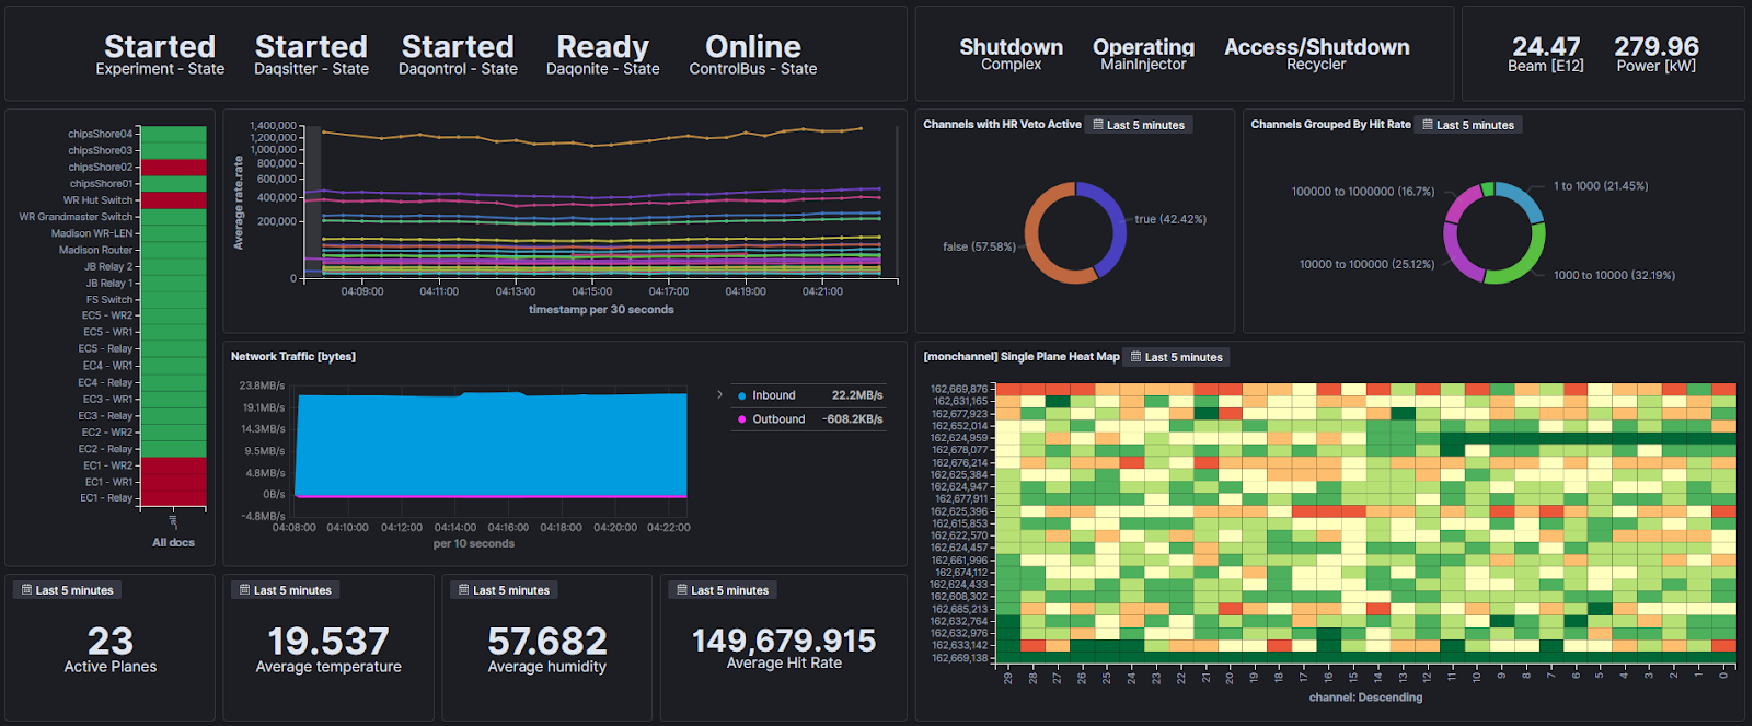
\includegraphics[width=\textwidth]{diagrams/5-daq/monitoring.pdf}
    \caption[monitoring short]
    {monitoring long}
    \label{fig:monitoring}
\end{figure}